\section{PERFORMANCE EVALUATION}
\label{sec: Performance Evaluation}

This section offers a comprehensive evaluation of the proposed solution, OmniFORE, detailing the dataset used, the benchmark SoA algorithms, the experimental setup, a multitude of evaluation scenarios, and an in-depth discussion of the results obtained.

\subsection{Benchmark Schemes}

The proposed model is evaluated against several high-performance algorithms designed to handle complex temporal and spatial dependencies in multivariate time-series data:

\subsubsection*{\textbf{LSTNet: Modeling Long- and Short-Term Temporal Patterns with Deep Neural Networks \cite{LSTNet}}}
LSTNet integrates CNNs and RNNs to capture both long-term and short-term patterns. It features a recurrent-skip component for modeling long-term dependencies and an autoregressive component to manage scale insensitivity.

\subsubsection*{\textbf{AGCRN: Adaptive Graph Convolutional Recurrent Network for Traffic Forecasting \cite{AGCRN}}}
AGCRN employs GCNs with trace-specific parameter learning and data-adaptive graph generation. This model dynamically adapts to specific patterns, excelling in various time-series forecasting tasks without requiring pre-defined graphs.


\subsection{Dataset}
\label{sec:Dataset}

The Google-Trace dataset \cite{google2019cluster} offers CPU and memory usage records from eight super cells (A-H) for May 2019, sampled every 5 minutes. Each cell contains 10,000 machines running thousands of containers, capturing diverse usage patterns critical for edge-cloud modeling and forecasting.

To rigorously evaluate our model's generalization capabilities, we partition the Google traces into two distinct sets: the \textbf{regular set} and the \textbf{zero-shot set}. The zero-shot set includes entirely new, previously unseen data, ensuring that the model has no prior exposure during training. This methodology prevents data leakage from the training set into the test set, providing a more accurate assessment of the model's generalization performance. Specifically, the model is trained on the regular set and then evaluated on the zero-shot set. Consequently, the results obtained from the zero-shot set more accurately represent the model's ability to generalize to novel, unseen data.

The regular set, composed of the \textbf{cells A-F}, is used for regular training, validation, and testing. In contrast, the zero-shot set, composed of the \textbf{cells G and H}, is reserved exclusively for zero-shot testing.

We selected 100 traces for each set to balance computational feasibility with the available hardware for training the models. This choice allows us to evaluate model performance accurately without overwhelming computational resources. The time dimension $d_t$ of the dataset was then split into training ($d_\text{train} = 0.6$), validation ($d_\text{val} = 0.2$), and test sets ($d_\text{test} = 0.2$). For a visual representation of the trace selection process, refer to Fig.~\ref{fig:proposed_solution_trace_selection}.

\subsection{Experimental Settings}
This section introduces the adopted model hyperparameters, the experimental environment, and the evaluation metrics.

\subsubsection{\textbf{Hyperparameters}}
We employ the Bayesian optimization technique described in Section \ref{sec:BayesianOptimizationWithGeneralizationObjective} to fine-tune the hyperparameters for the different models. Table \ref{table:hyperparameters} presents the hyperparameter ranges and optimized values for OmniFORE, AGCRN, and LSTNet models. These ranges, based on the original authors' recommendations \cite{AGCRN, LSTNet}, strike a balance between exploration and practicality to achieve optimal generalization across diverse datasets. The Bayesian optimization process began with 20 initial training runs, followed by 30 iterations to refine the hyperparameters. The optimal hyperparameter values for the different models are listed in the result column of Table \ref{table:hyperparameters}.

\subsubsection{\textbf{Hardware and Software Environment}}
All experiments are conducted on a server equipped with 1x NVIDIA A100 SXM GPU (40 GB memory), 30 CPU cores, 200 GiB RAM, and 512 GiB SSD. The server uses an Intel Xeon processor and runs Ubuntu 20.04.2 LTS with the GNU/Linux 5.4.0-70-generic x86\_64 kernel. All methods are implemented in Python. The LSTNet and AGCRN models, provided by their authors, have been re-implemented using PyTorch 3.2.1.

\begin{table}
\centering
\caption{Hyperparameter Ranges for Bayesian Optimization Per Model}
\label{table:hyperparameters}
\footnotesize
\begin{tabular}{|c|l|c|c|c|}
\hline
\textbf{} & \textbf{Hyperparameter}       & \textbf{Symbol} & \textbf{Range}  & \textbf{Result} \\
\hline
\multirow{10}{*}{\rotatebox{90}{OmniFORE}} 
 & Model dimension           & $d_{embed}$   & (64, 512)  & 194 \\
 & Sequence length           & $d_x$        & (24, 256)  & 98  \\
 & Prediction length         & $d_y$        & (12, 64)   & 14  \\
 & Dropout rate              & $h_{1}$      & (0.15, 0.4) & 0.161 \\
 & Feedforward dim.          & $h_{2}$      & (128, 512) & 356 \\
 & Encoder layers            & $h_{3}$      & (1, 4)     & 2   \\
 & Decoder layers            & $h_{4}$      & (1, 3)     & 1   \\
 & Attention heads           & $h_{5}$      & (4, 16)    & 6   \\
 & Label length              & $h_{6}$      & (32, 64)   & 48  \\
 & Batch size                & $h_{7}$     & (16, 64)   & 47  \\
\hline
\multirow{7}{*}{\rotatebox{90}{AGCRN}} 
 & Embedding  dim.       & $d_{embed}$  & (2, 30)    & 3   \\
 & Sequence length           & $d_x$        & (12, 72)   & 48  \\
 & Prediction length         & $d_y$        & (12, 72)   & 22  \\
 & RNN units                 & $h_{8}$     & (50, 200)  & 76  \\
 & Number of layers          & $h_{9}$     & (1, 3)     & 1   \\
 & Chebyshev order & $h_{14}$    & (1, 3)     & 1   \\
 & Batch size                & $h_{10}$     & (16, 64)   & 25  \\
\hline
\multirow{10}{*}{\rotatebox{90}{LSTNet}} 
 & Sequence length           & $d_x$        & (144, 192) & 161 \\
 & Prediction length         & $d_y$        & (6, 12)    & 11  \\
 & Dropout rate              & $h_{11}$     & (0.1, 0.2) & 0.13 \\
 & CNN hidden units          & $h_{12}$     & (20, 143)  & 50  \\
 & RNN hidden units          & $h_{13}$     & (20, 143)  & 107 \\
 & CNN kernel size           & $h_{14}$     & (6, 18)    & 14  \\
 & Highway window size       & $h_{15}$     & (24, 168)  & 93  \\
 & Batch size                & $h_{16}$     & (16, 64)   & 33  \\
 & Skip length               & $h_{17}$     & (24, 24)   & 24  \\
 & Skip hidden units         & $h_{18}$     & (20, 100)  & 77  \\
\hline
\end{tabular}
\end{table}


\subsubsection{\textbf{Evaluation Metrics}}
The performance of all schemes is evaluated considering the following metrics.

\paragraph*{Mean Absolute Error (MAE)}
This metric measures the average magnitude of errors without considering their direction, making it useful for assessing overall accuracy. The MAE is calculated as
\begin{equation}
  \text{MAE} = \frac{1}{n \times d_y} \sum_{i=1}^{n} \sum_{t=1}^{d_y} \left| \hat{T}_i(t) - T_i(t) \right|.
\end{equation}

\paragraph*{Root Mean Square Error (RMSE)}
This metric highlights larger errors, making it particularly effective for datasets with significant fluctuations. The RMSE is given by
\begin{equation}
  \text{RMSE} = \sqrt{\frac{1}{n \times d_y} \sum_{i=1}^{n} \sum_{t=1}^{d_y} \left( \hat{T}_i(t) - T_i(t) \right)^2}.
\end{equation}

\paragraph*{Symmetric Mean Absolute Percentage Error (SMAPE)}
This percentage-based metric is useful for comparing accuracy across different scales. The SMAPE is defined as
\begin{equation}
  \text{SMAPE} = 2 \cdot \frac{100\%}{n \times d_y} \sum_{i=1}^{n} \sum_{t=1}^{d_y} \frac{\left| \hat{T}_i(t) - T_i(t) \right|}{\left( \left| \hat{T}_i(t) \right| + \left| T_i(t) \right| \right)}.
\end{equation}

\paragraph*{Inference Time}
Inference time refers to the average duration the model requires to process its inputs and generate an output. This metric is crucial for applications demanding real-time predictions.

\paragraph*{Convergence Speed}
Convergence speed evaluates how quickly a model's training process stabilizes. A patience parameter of three is employed, ceasing training if the validation loss does not improve over three epochs. Performance is assessed using the test set RMSE after convergence to ensure robust generalization to unseen data. Lower metric values indicate better performance, providing a comprehensive evaluation of prediction accuracy and reliability.

\subsection{Experimental Results}
\label{sec: Experimental Results}

In this section, we present our evaluation results, demonstrating that the proposed model outperforms existing algorithms across all criteria. OmniFORE consistently shows lower error rates, better generalization on new data, and faster inference times. It is minimally impacted by dynamic workload changes and effectively handles trace variance, maintaining lower errors in diverse scenarios. Additionally, OmniFORE converges faster than current algorithms, highlighting its robustness and efficiency.

\subsubsection{\textbf{Hyperparameter Sensitivity and Optimization Effectiveness}}

We evaluate the sensitivity of the models to hyperparameters to gauge the effectiveness of our optimization approach from Section \ref{sec:BayesianOptimizationWithGeneralizationObjective}. Using the hyperparameter ranges $h_i$ specified in Table \ref{table:hyperparameters}, we measure performance. Figure \ref{fig:test_rmse_distribution_histogram} depicts the effect of hyperparameter tuning on test RMSE for OmniFORE, AGCRN, and LSTNet models.

OmniFORE achieves a mean test RMSE of $2.99 \times 10^{-4}$ with a standard deviation of $7.22 \times 10^{-4}$, and a factor difference (max/min) of 38.45. AGCRN records a mean test RMSE of $4.56 \times 10^{-4}$ with a standard deviation of $7.89 \times 10^{-4}$. LSTNet reports a mean test RMSE of $5.78 \times 10^{-4}$ and a standard deviation of $1.25 \times 10^{-3}$.

OmniFORE exhibits the lowest mean test RMSE and standard deviation, suggesting superior performance and reduced sensitivity to hyperparameters. However, precise tuning enhances OmniFORE's performance by a factor of 38.45, underscoring the significance of our custom Bayesian optimization for achieving robust generalization.

\begin{figure}%[H]
\centering
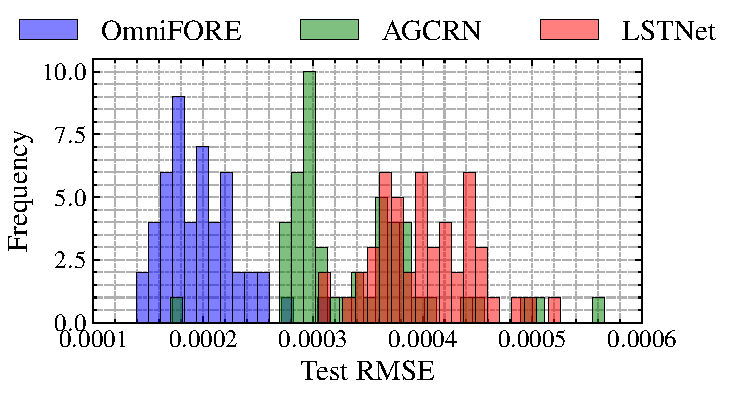
\includegraphics[width=0.49\textwidth]{img/test_rmse_distribution_histogram.pdf}
\caption{Sensitivity to Hyperparameters for Model Generalization}
\label{fig:test_rmse_distribution_histogram}
\end{figure}

\subsubsection{\textbf{Generalization Performance}}
\label{sec: Evaluation - Generalization Performance}
\paragraph*{Regular Training}
Figure \ref{fig:metrics_comparison_regular} displays the prediction performance of various models on test data from Google Cells A-F after regular training. OmniFORE demonstrates superior performance over AGCRN and LSTNet across all evaluation metrics.

OmniFORE achieves an MAE of $8.53 \times 10^{-4}$, RMSE of $5.50 \times 10^{-3}$, and SMAPE of 11.21\%. In contrast, AGCRN records an MAE of $1.04 \times 10^{-3}$, RMSE of $5.98 \times 10^{-3}$, and SMAPE of 37.19\%. LSTNet reports an MAE of $2.10 \times 10^{-3}$, RMSE of $9.21 \times 10^{-3}$, and SMAPE of 23.52\%. OmniFORE's MAE is 18.21\% lower than AGCRN and 59.42\% lower than LSTNet. Its RMSE is 7.97\% lower than AGCRN and 40.21\% lower than LSTNet. OmniFORE's SMAPE is 69.86\% lower than AGCRN and 52.34\% lower than LSTNet. This notable improvement is attributed to OmniFORE's advanced attention mechanism, which captures both long-term and short-term correlations among workloads.

Furthermore, OmniFORE achieves these results with an average inference time of \SI{8.70}{\milli\second}, compared to \SI{131}{\milli\second} for AGCRN and \SI{10.6}{\milli\second} for LSTNet. This represents a 17.92\% reduction in inference time compared to the best-performing SoA scheme, highlighting OmniFORE's efficiency for real-time applications where quick orchestration decisions are required with minimal resource overhead \cite{9500858, 8334540}. This efficiency is thanks to OmniFORE's use of generative inference, which predicts the entire sequence in a single step rather than sequentially.

\begin{figure}%[H]
\centering
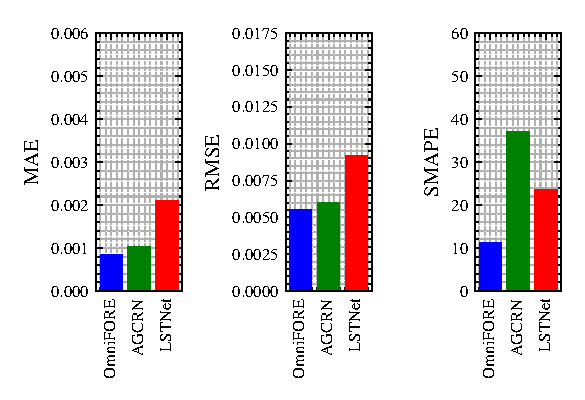
\includegraphics[width=0.49\textwidth]{img/metrics_comparison_regular.eps}
\caption{Generalization performance comparison of MAE, RMSE and SMAPE for each model for the \textbf{regular training} traces.}
\label{fig:metrics_comparison_regular}
\end{figure}

\paragraph*{Zero-Shot Performance}
Figure \ref{fig:metrics_comparison_ZS} illustrates the prediction performance using zero-shot test data from Google Cells G and H. OmniFORE achieves an MAE of $6.34 \times 10^{-4}$, RMSE of $2.92 \times 10^{-3}$, and SMAPE of 6.31\%. In comparison, AGCRN records an MAE of $3.93 \times 10^{-3}$, RMSE of $9.65 \times 10^{-3}$, and SMAPE of 55.27\%, while LSTNet shows an MAE of $5.02 \times 10^{-3}$, RMSE of $1.49 \times 10^{-2}$, and SMAPE of 39.91\%.

OmniFORE's superior zero-shot performance, surpassing even its regular training performance, stems from its advanced attention-based mechanism that captures complex patterns and dependencies, enabling robust generalization. In contrast, AGCRN and LSTNet perform worse on zero-shot data, indicating potential benefits from information leakage between training and test sets. Additionally, data variability and the exact nature of loaded traces can influence performance outcomes.

\begin{figure}%[H]
\centering
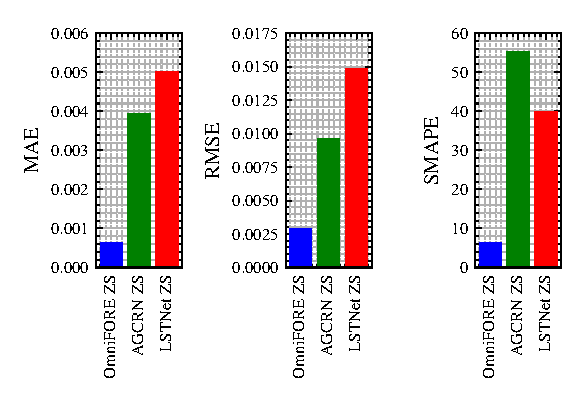
\includegraphics[width=0.42\textwidth]{img/metrics_comparison_zs.eps}
\caption{Generalization performance comparison of MAE, RMSE, and SMAPE for each model on the \textbf{zero-shot} traces.}
\label{fig:metrics_comparison_ZS}
\end{figure}


\subsubsection{\textbf{Impact of Prediction Length on Inference Time}}

In the millisecond regime, longer prediction lengths are particularly advantageous \cite{9500858}. Short-term predictions require frequent adjustments, leading to higher computational overhead and inefficiencies. In contrast, longer-term predictions enhance stability and responsiveness, allowing for smoother and more strategic resource management. This reduces the need for constant real-time recalibration and optimizes overall performance in edge-cloud environments.

As shown in Figure \ref{fig:pred_vs_inf}, we study the inference time (left subplot) and the performance in terms of RMSE (right subplot) over different prediction lengths. The inference time subplot reveals that LSTNet's computation time significantly increases with prediction length, reaching \SI{240}{\milli\second} for a length of 300, making it unsuitable for real-time applications that require latency within the \SI{50}{\milli\second} limit \cite{8334540}. In contrast, OmniFORE maintains low inference times, from \SI{12.7}{\milli\second} for a length of 5 to \SI{34}{\milli\second} for 300, thanks to efficient attention mechanisms and fast decoding. AGCRN's inference time also rises with longer predictions, reaching \SI{56}{\milli\second} for 300, which exceeds the real-time requirement, but remains higher than OmniFORE. Overall, OmniFORE is approximately twice as fast as AGCRN across all prediction lengths while maintaining performance, as evidenced by the RMSE results in the right subplot.

OmniFORE consistently outperforms AGCRN and LSTNet in RMSE, demonstrating superior accuracy. AGCRN's RMSE is generally low performant. OmniFORE's combination of low inference time and high accuracy makes it ideal for real-time, dynamic applications, outperforming both AGCRN and LSTNet.

\begin{figure}%[H]
\centering
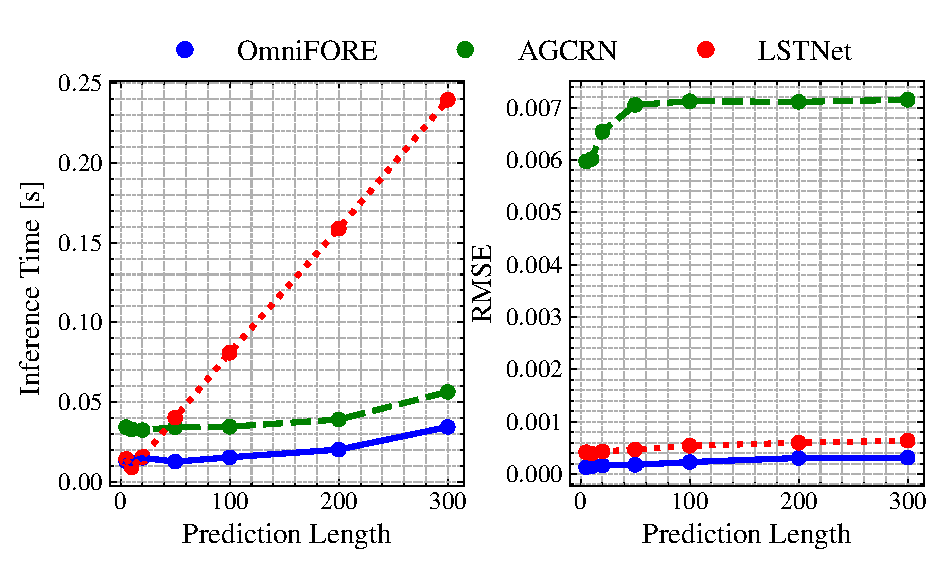
\includegraphics[width=0.42\textwidth]{img/pred_vs_inf.eps}
\caption{Impact of prediction length on inference time and RMSE for OmniFORE, AGCRN, and LSTNet.}
\label{fig:pred_vs_inf}
\end{figure}
\subsubsection{\textbf{Periodic Dynamic Workload Changes with Long-term Dependencies}}

To rigorously test OmniFORE's attention mechanism and its capacity to capture long-range dependencies, we design a signal with frequent, highly dynamic changes based on the workload diversity described in Section~\ref{sec: System Model} (Fig. \ref{fig:dynamic_workload_changes}). The signal's periodic nature, alternating between low and high usage over extended cycles, challenges the model to recognize and utilize information from distant time steps, rigorously evaluating its long-term pattern recognition capabilities.

The workload components are defined as 
\begin{equation}
T(t) = \mu \left( \sin(2\pi f t) \cdot \mathbf{1}_{\{t \% (1/f) < 0.5\}} + \mathcal{N}(0, \sigma) \right),
\end{equation}
where $\mu$ represents the mean value for the workload, $f$ is the frequency, and $\sigma$ is the standard deviation. The indicator function $\mathbf{1}_{\{t \% (1/f) < 0.5\}}$ ensures that the sine wave is active for half of its period. $\mathcal{N}(0, \sigma)$ represents Gaussian noise with a mean of 0 and standard deviation $\sigma$. The overall workload signal is generated by combining a low and high workload component:
\begin{equation}
T(t) = \begin{cases} 
T_{\text{low}}(t), & \text{if } t < \text{pattern\_length} / 2 \\
T_{\text{high}}(t), & \text{otherwise}
\end{cases}
\end{equation}
where pattern\_length = 48, representing a 2-hour cycle with 5-minute intervals.
For the low workload component, $\mu_{\text{low}} = 0.01$, $f_{\text{low}} = 0.5$, and $\sigma_{\text{low}} = 0.002$. For the high workload component, $\mu_{\text{high}} = 0.08$, $f_{\text{high}} = 1.0$, and $\sigma_{\text{high}} = 0.01$. The final workload is then adjusted to ensure positive values:

\begin{equation}
T_{\text{final}}(t) = T(t) + \mu_{\text{low}}.
\end{equation}

The connection between these equations and the input sequence lengths ($d_x$) lies in the periodic nature of the generated data. Each data point represents a 5-minute interval, making the input sequence lengths for OmniFORE (98 intervals), AGCRN (48 intervals), and LSTNet (161 intervals) (see Table \ref{table:hyperparameters}), adequate to capture the recurring patterns of the workload cycles.

Analysis of OmniFORE, AGCRN, and LSTNet reveals that OmniFORE consistently outperforms the other models. OmniFORE achieves an RMSE of 0.0322, compared to 0.0440 for AGCRN and 0.0806 for LSTNet. The lower RMSE indicates that OmniFORE's predictions have smaller average deviations from the true values, demonstrating its superior accuracy in capturing the dynamic workload patterns.

OmniFORE's advanced attention mechanism demonstrates a superior ability to understand long-term dependencies, enabling it to accurately predict dynamic changes in the workload. This capability is evident in its precise anticipation of transitions between low and high workload periods. In contrast, AGCRN and LSTNet exhibit limitations in capturing these long-range patterns, resulting in greater deviations from the true values, particularly during workload transitions. LSTNet's performance is hindered by its inability to effectively model dependencies beyond approximately 40 data points, a consequence of the vanishing gradient problem \cite{zhou2021informer}. Similarly, the CNN-based approach employed by AGCRN struggles with long-range dependencies \cite{acmtimeseriesreview2024, hochreiter1998vanishing}, impeding its ability to accurately capture and predict extended periodic patterns in the workload signal.

Notably, even in the low workload regions of the signal, OmniFORE demonstrates an understanding of the existence of minor peaks, showcasing its ability to capture fine-grained patterns in the data.

\begin{figure}
\centering
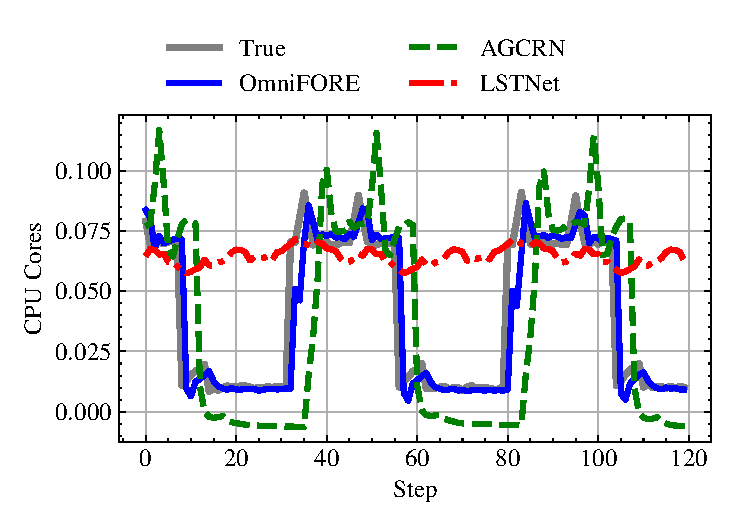
\includegraphics[width=0.42\textwidth]{img/dynamic_workload_changes.eps}
\caption{Comparison of true and predicted values for OmniFORE, AGCRN, and LSTNet under dynamic workload changes.}
\label{fig:dynamic_workload_changes}
\end{figure}

\subsubsection{\textbf{Variance-based Performance}}

We compare OmniFORE, AGCRN, and LSTNet models on both the regular CPU cores dataset and the zero-shot dataset introduced in Section \ref{sec: Evaluation - Generalization Performance} to assess their capacity to handle data with heterogeneous variance levels (Figure \ref{fig:zs_sample_trace_comparison}). OmniFORE demonstrates superior performance in capturing both low and high variance patterns, evidenced by its closer alignment with true values across diverse trace volatilities. This advantage is particularly pronounced in highly fluctuating traces, where OmniFORE maintains accuracy while AGCRN and LSTNet show increased deviations. The consistent performance of OmniFORE across both datasets underscores its robust generalization capabilities, effectively adapting to previously unseen patterns in the zero-shot scenario. 

\begin{figure}%[H]
\centering
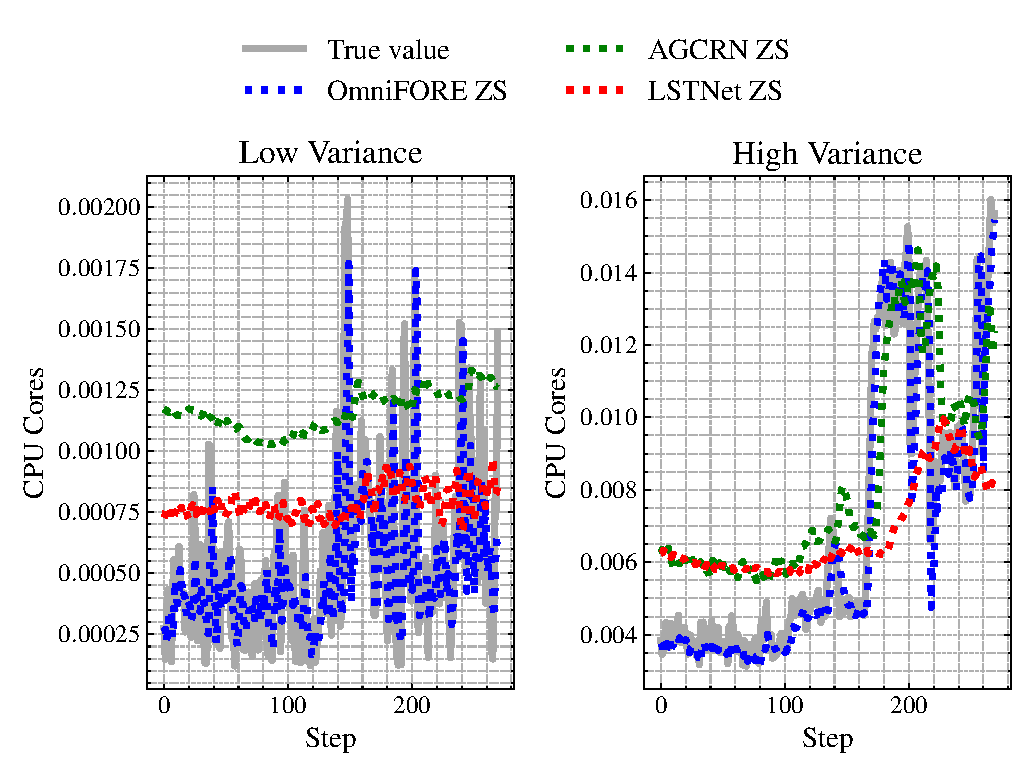
\includegraphics[width=0.42\textwidth]{img/zs_sample_trace_comparison.eps}
\caption{Comparison of true and \textbf{zero-shot} predicted values for OmniFORE, AGCRN, and LSTNet on a regular training dataset.}
\label{fig:zs_sample_trace_comparison}
\end{figure}

To further investigate, we measured the variance of each individual test trace $T_{\text{val}, i}$ and computed the performance metrics (MAE and RMSE) for these traces. Figure \ref{fig:metrics_variance_comparison_fitted} shows the relationship between trace variance and performance metrics, with linear trend lines fitted to highlight trends.

In Figure \ref{fig:metrics_variance_comparison_fitted}, slopes indicate error increase rates with rising input variance. OmniFORE exhibits the lowest slopes (regular: $1.19 \times 10^2$, zero-shot: $2.32 \times 10^1$), outperforming AGCRN (regular: $1.36 \times 10^2$, zero-shot: $2.24 \times 10^2$) and LSTNet (regular: $2.60 \times 10^2$, zero-shot: $8.75 \times 10^2$). This demonstrates OmniFORE's superior robustness to high-variance data, particularly in zero-shot scenarios.

We evaluate OmniFORE, AGCRN, and LSTNet on low and high variance traces in both regular and zero-shot scenarios. For the five lowest variance traces, OmniFORE-regular achieves an MAE of $8.96 \times 10^{-7}$, outperforming AGCRN-regular ($1.49 \times 10^{-4}$) and LSTNet-regular ($2.30 \times 10^{-6}$) by 99.4\% and 61.0\% respectively. On high variance traces, OmniFORE-regular (MAE: $1.00 \times 10^{-2}$) surpasses LSTNet-regular ($2.44 \times 10^{-2}$) by 59.0\%. In the zero-shot scenario with high variance traces, OmniFORE (MAE: $3.01 \times 10^{-3}$) outperforms AGCRN ($4.26 \times 10^{-3}$) and LSTNet ($9.05 \times 10^{-3}$) by 29.3\% and 66.7\% respectively. These results demonstrate OmniFORE's consistent superiority across diverse variance levels and generalization scenarios.

\begin{figure}%[H]
\centering
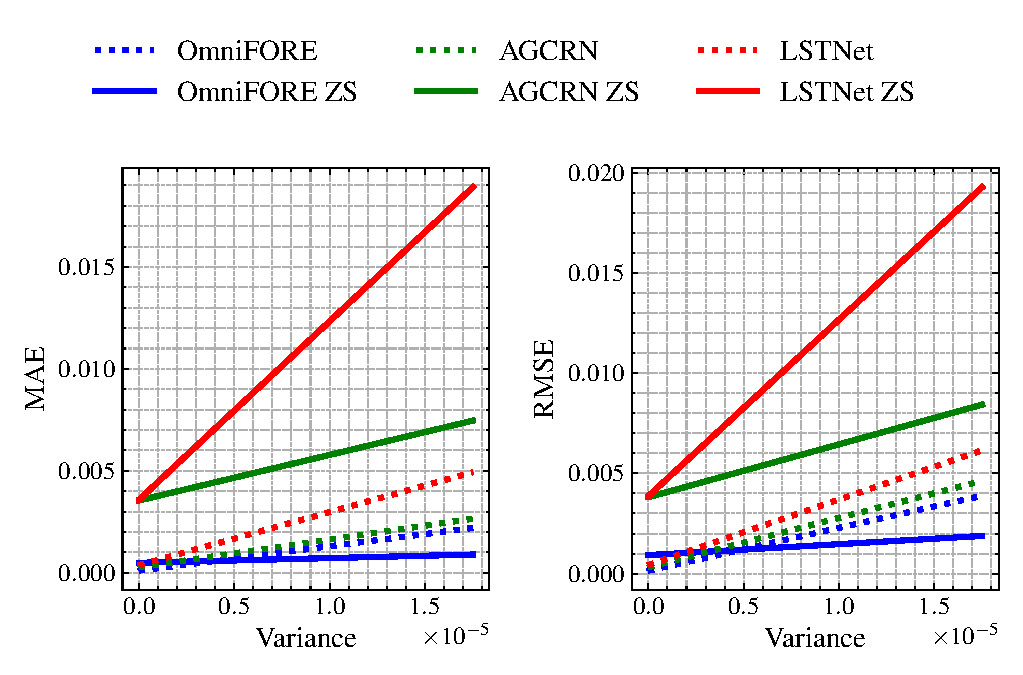
\includegraphics[width=0.47\textwidth]{img/metrics_variance_comparison_fitted2.eps}
\caption{Trace variance vs. MAE and RMSE for OmniFORE, AGCRN, and LSTNet models, with fitted linear lines.}
\label{fig:metrics_variance_comparison_fitted}
\end{figure}

\subsubsection{\textbf{Convergence}}

Quick model convergence is crucial to reduce the need for extensive training, which aids in deploying updates and maintaining overall system performance. Additionally, models that converge faster are less prone to overfitting, as they achieve their optimal state in fewer epochs.

Figure \ref{fig:test_rmse_convergence_comparison} depicts the test RMSE convergence of OmniFORE, AGCRN, and LSTNet models over multiple epochs, with early stopping applied.

OmniFORE demonstrates the fastest convergence, achieving the lowest RMSE of $5.3 \times 10^{-3}$ by the 6th epoch. LSTNet converges more gradually, reaching $8.8 \times 10^{-3}$ by the 8th epoch. AGCRN exhibits the slowest convergence, reaching $6.0 \times 10^{-3}$ by the 16th epoch.

\begin{figure}%[H]
\centering
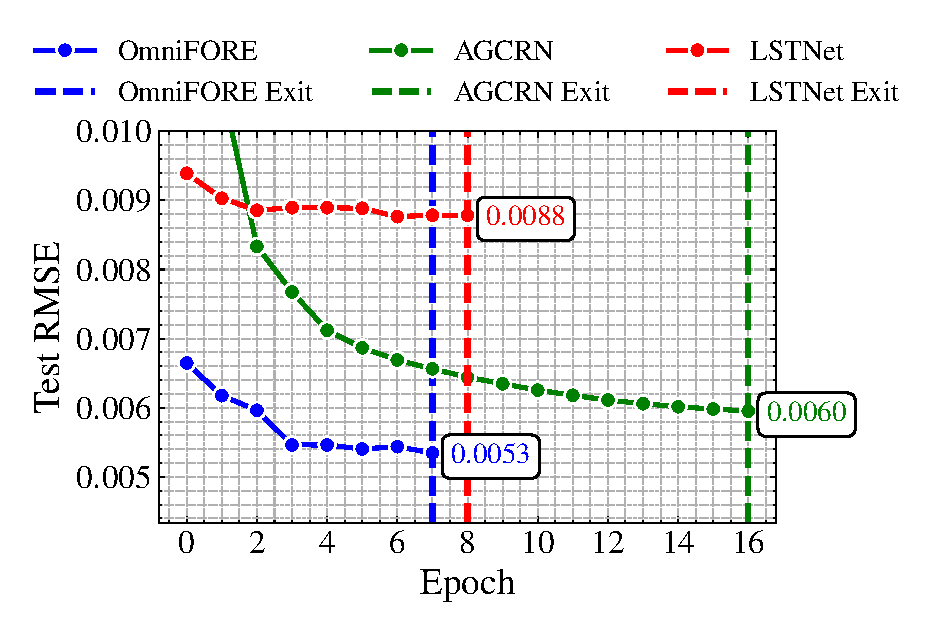
\includegraphics[width=0.49\textwidth]{img/test_rmse_convergence_comparison.eps}
\caption{Convergence of OmniFORE, AGCRN, and LSTNet models over epochs.}
\label{fig:test_rmse_convergence_comparison}
\end{figure}

% \subsection{Practical Edge-cloud Machine Learning Deployment}
% \label{sec:edge_cloud_orchestration}

% We present an advanced edge-cloud orchestration system for scalable machine learning deployment, inference, and real-time decision-making (Fig. \ref{fig:Practical_Scenario}). This architecture integrates edge computing with cloud infrastructure, optimizing both computational efficiency and resource allocation.

% \begin{figure}[t]
% \centering
% 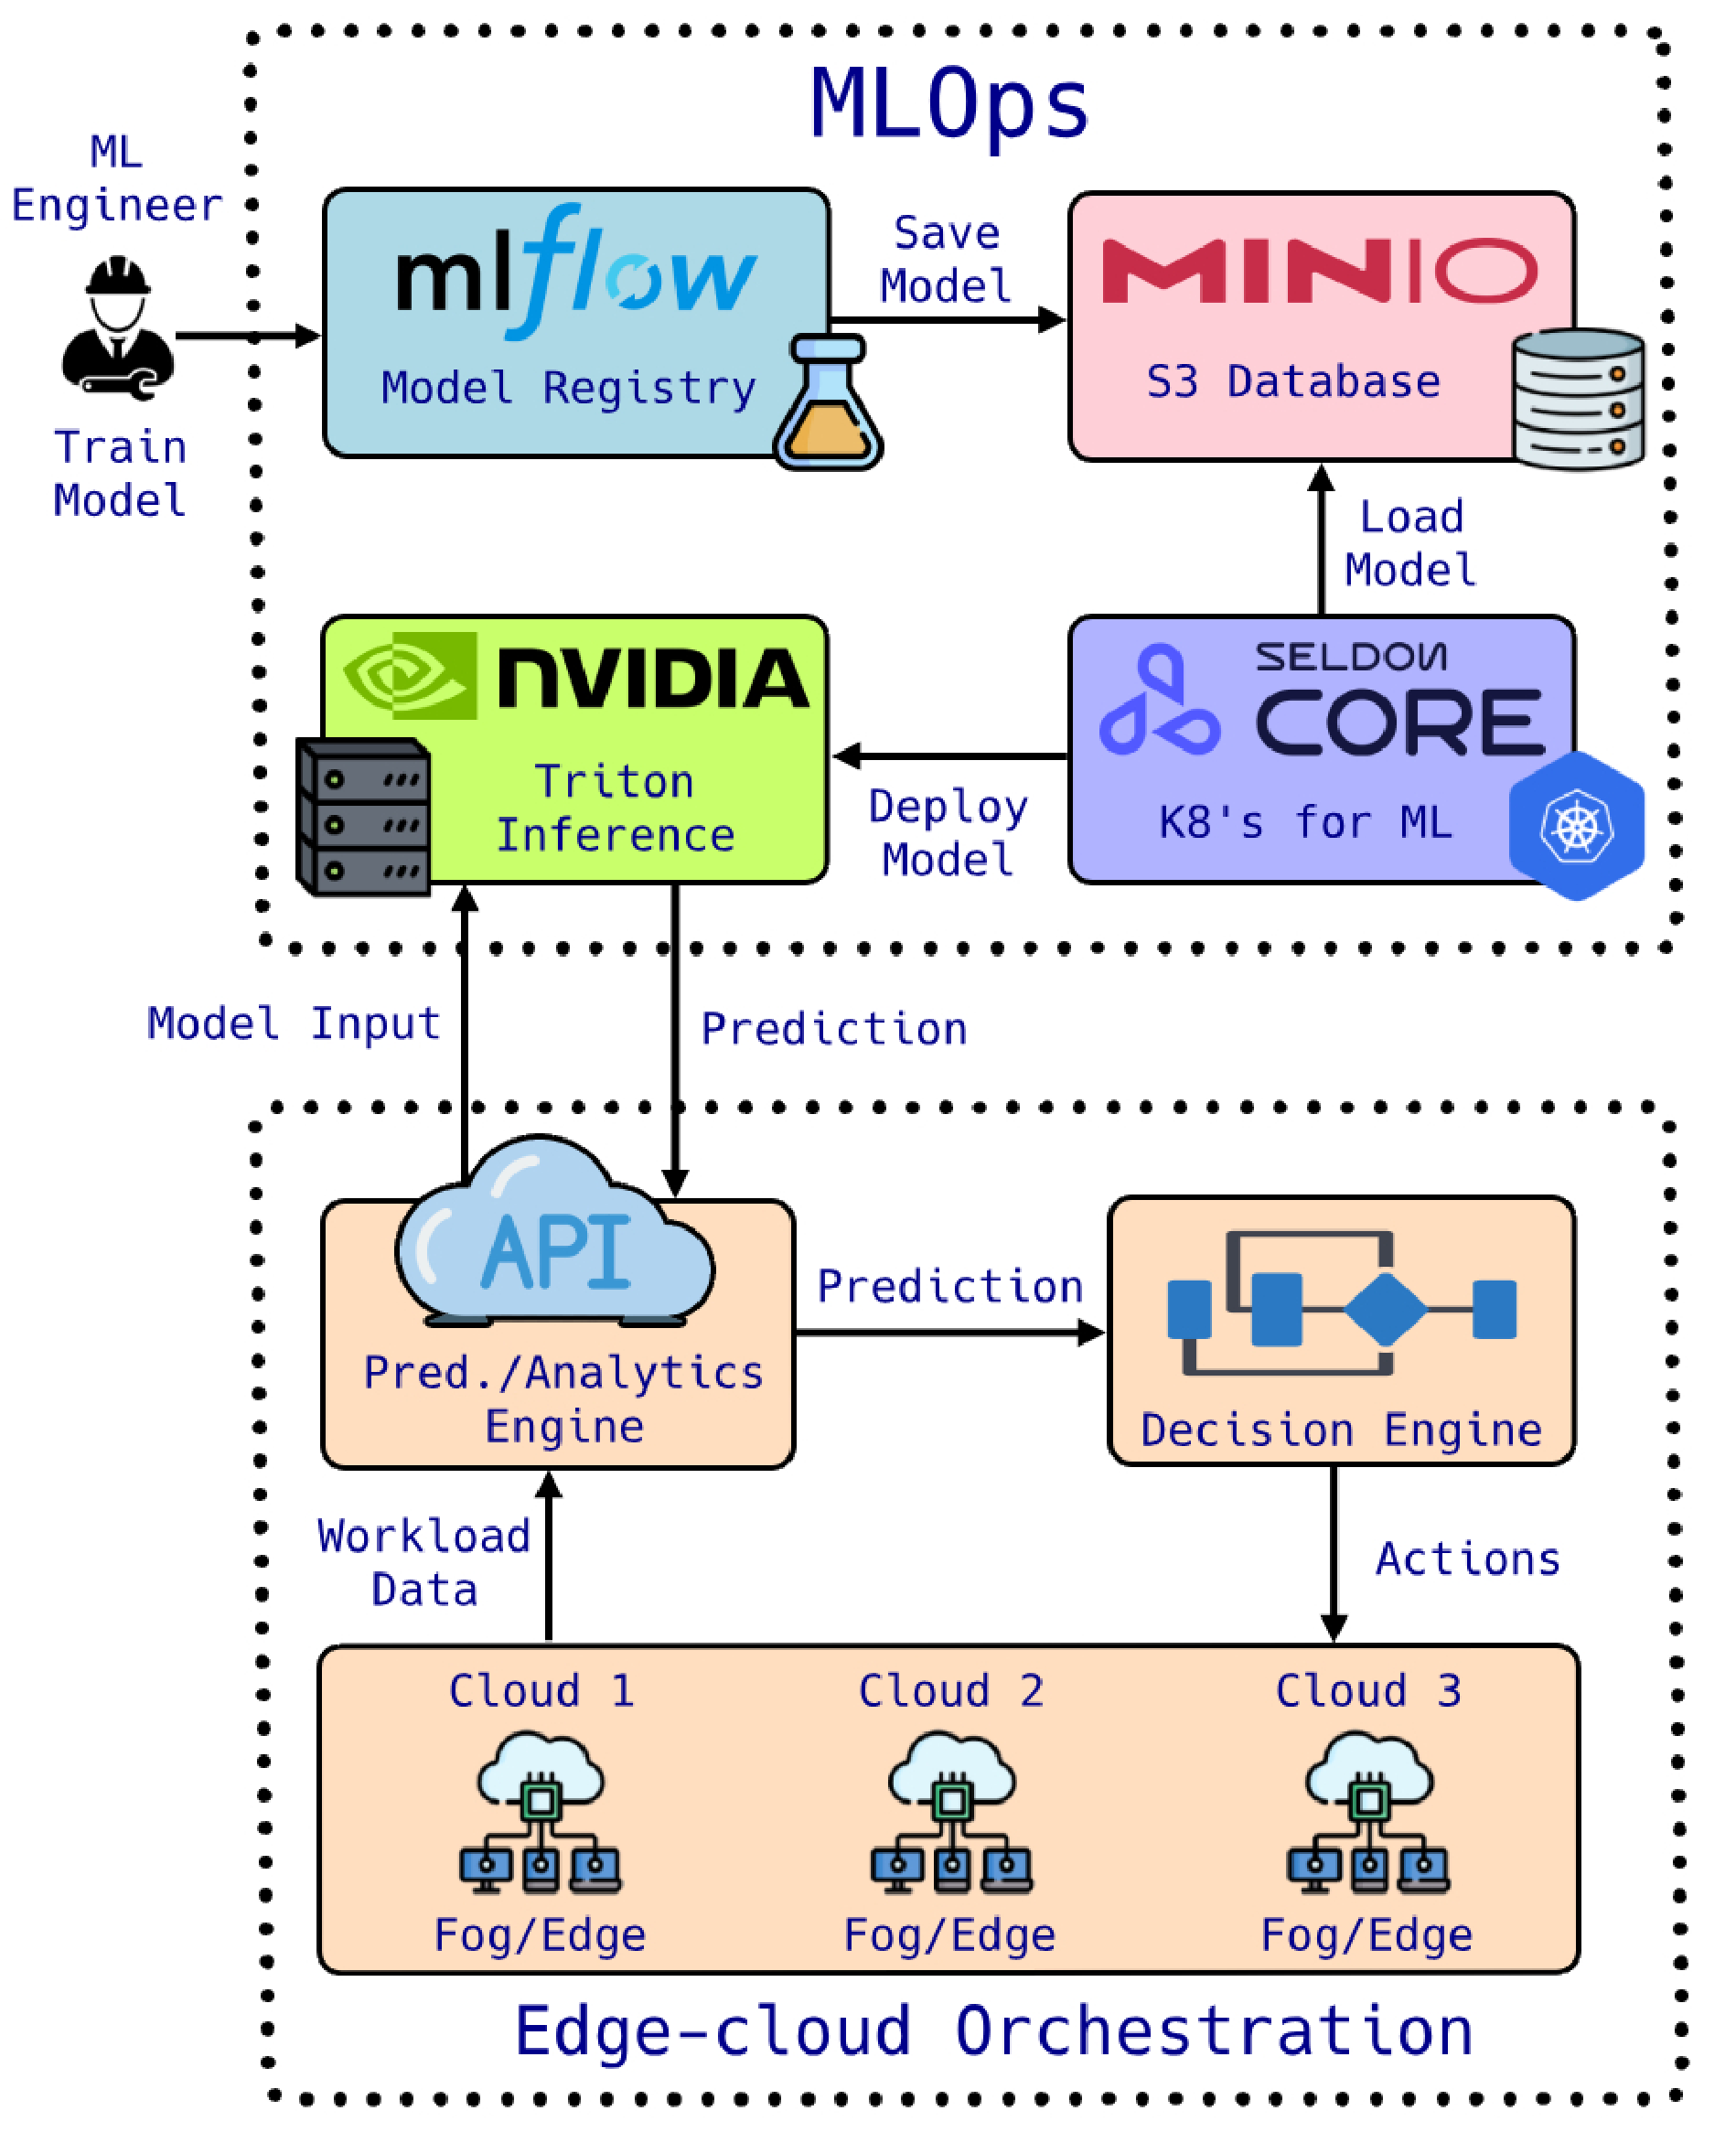
\includegraphics[width=0.47\textwidth]{img/Practical_Scenario.pdf}
% \caption{Scalable ML deployment and inference for Edge-cloud orchestration.}
% \label{fig:Practical_Scenario}
% \end{figure}

% \subsubsection{Model Development and Registry}

% Our system employs MLflow as the Model Registry, integrated with S3-compatible storage. MLflow provides robust versioning, comprehensive metadata management, and seamless integration with MLOps frameworks, facilitating reproducibility and smooth transitions from development to production across various ML frameworks.

% \subsubsection{Orchestration and Deployment}

% Kubernetes serves as the orchestration layer, managing deployment and scaling of our ML infrastructure. It offers efficient container orchestration, resource optimization, and self-healing capabilities, ensuring system reliability and scalability.

% \subsubsection{Scalable Inference}

% Scalable inference is achieved through a combination of NVIDIA Triton Inference Server and Seldon Core. Triton provides high-performance, GPU-accelerated inference with multi-framework support. It excels in concurrent model execution, dynamic batching, and supports model pipelines. Triton's HTTP/REST and gRPC inference protocols ensure broad compatibility and efficient communication.

% Seldon Core complements Triton by providing Kubernetes-native deployment for production-grade ML serving. It enables multi-model serving with efficient resource utilization, complex inference pipelines, and A/B testing capabilities. Seldon Core also offers explanation mechanisms and monitoring for deployed models.

% This combination allows for efficient deployment of diverse models from edge to cloud while maintaining high performance and scalability. A single model endpoint can serve thousands of fog/edge nodes simultaneously. This is achieved through Triton's optimized performance for various query types, combined with Seldon's ability to overcommit resources by deploying more models than available memory and unloading inactive models as needed. The result is a system capable of handling high-throughput requests from numerous edge devices efficiently.

% \subsubsection{Edge and Cloud Integration}

% Fog/Edge Nodes perform initial data processing and lightweight inference to reduce latency and minimize data transfer. Cloud Servers handle more complex computations and large-scale data analysis. A Prediction/Analytics Engine aggregates insights from both edge and cloud components, feeding into a Decision Engine for real-time decision-making.

% This architecture enables efficient, scalable, and flexible ML deployment across diverse computing environments, from resource-constrained edge devices to powerful cloud infrastructure. By leveraging Triton and Seldon Core, our system can efficiently manage thousands of fog/edge nodes from centralized model endpoints, balancing edge responsiveness with cloud computing power. The result is a robust, scalable system capable of meeting the demands of modern ML deployment scenarios across a wide range of applications and environments.